%%%%%%%%%%%%%%%%%%%%%%%%%%%%%%%%%%%%%%%%%%%%%%%%%%%%%%%%%%%%
\subsubsection*{Neutrinoless double beta decay and Majorana neutrinos}

Neutrinos, unlike the other Standard Model fermions, could be Majorana particles, that is, indistinguishable from their antiparticles. The existence of Majorana neutrinos would have profound implications in particle physics and cosmology. If neutrinos are Majorana particles, there must exist a new scale of physics the level of which is inversely proportional to neutrino masses, that characterises new underlying dynamics beyond the Standard Model. The existence of such a new scale provides the simplest explanation of why neutrino masses are so much lighter than the charged fermions. Understanding the new physics that underlies neutrino masses is one of the most important open questions in particle physics. It could have profound implications in our understanding of the mechanism of symmetry breaking, the origin of mass and the flavour problem.

Furthermore, the existence of Majorana neutrinos would imply that lepton number is not a conserved quantum number which could be the origin of the matter-antimatter asymmetry observed in the Universe. The new physics related to neutrino masses could provide a new mechanism to generate the asymmetry, called leptogenesis. 

The only practical way to establish experimentally that neutrinos are their own antiparticle is the detection of neutrinoless double beta decay (\bbonu). This is a postulated very slow radioactive process in which a nucleus with $Z$ protons decays into a nucleus with $Z+2$ protons and the same mass number $A$, emitting two electrons that carry essentially all the energy released (\Qbb). The process can occur if and only if neutrinos are massive, Majorana particles.

Several underlying mechanisms --- involving, in general, physics beyond the Standard Model  --- have been proposed for \bbonu, the simplest one being the virtual exchange of light Majorana neutrinos. Assuming this to be the dominant process at low energies, the half-life of \bbonu\ can be written as
\begin{equation}
(T^{0\nu}_{1/2})^{-1} = G^{0\nu} \ \big|M^{0\nu}\big|^{2} \ \mbb^{2} \, .
\label{eq:Tonu}
\end{equation}
In this equation, $G^{0\nu}$ is an exactly-calculable phase-space integral for the emission of two electrons; $M^{0\nu}$ is the nuclear matrix element (NME) of the transition, which has to be evaluated theoretically; and \mbb\ is the \emph{effective Majorana mass} of the electron neutrino:
\begin{equation}
\mbb = \Big| \sum_{i} U^{2}_{ei} \ m_{i} \Big| \, ,
\end{equation}
where $m_{i}$ are the neutrino mass eigenstates and $U_{ei}$ are elements of the neutrino mixing matrix. Therefore, a measurement of the decay rate of \bbonu\ would provide direct information on neutrino masses.

The relationship between \mbb\ and the actual neutrino masses $m_i$ is affected by the uncertainties in the measured oscillation parameters, the unknown neutrino mass ordering (normal or inverted), and the unknown phases in the neutrino mixing matrix (both Dirac and Majorana). The current knowledge on neutrino masses and mixings provided by neutrino oscillation experiments is summarized in the left panel of fig.~\ref{fig:numass_ordering}. The diagram shows the two possible mass orderings that are compatible with neutrino oscillation data, with increasing neutrino masses from bottom to top. The relationship between \mbb\ and the lightest neutrino mass $m_{\rm light}$ (which is equal to $m_1$ or $m_3$ in the normal and inverted mass orderings, respectively) is illustrated in the right panel of Fig.~\ref{fig:numass_ordering}.

%%%%%%%%%%
\begin{figure}[h]
\centering
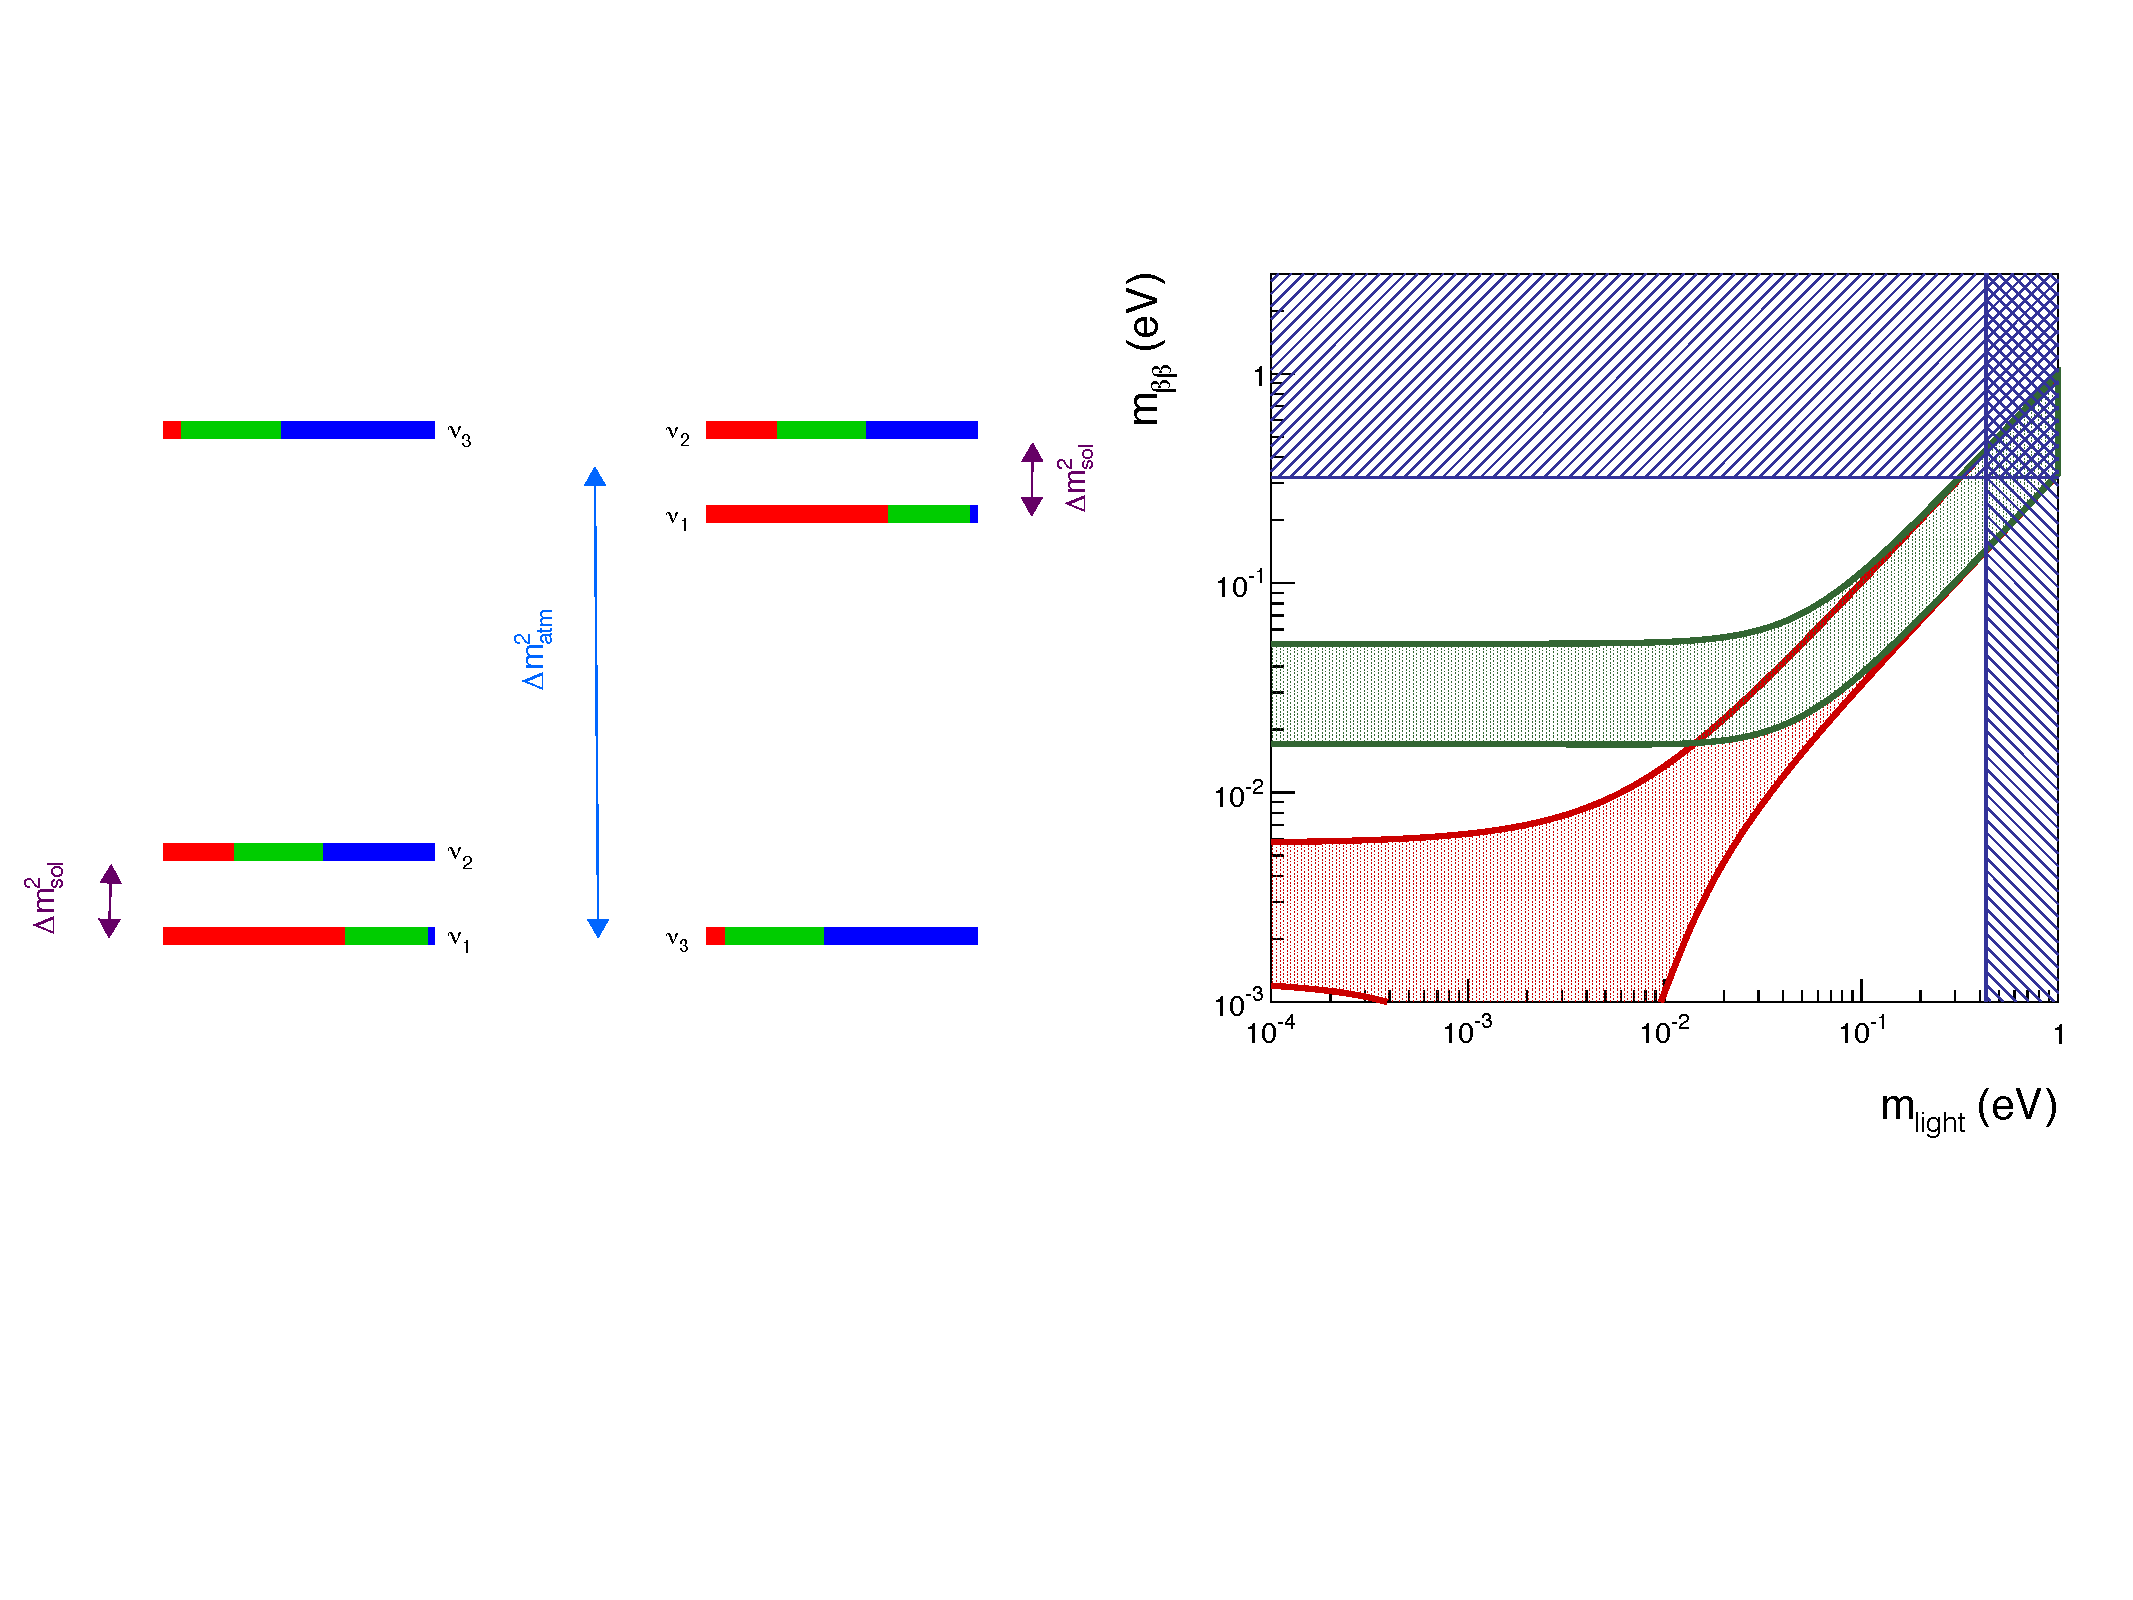
\includegraphics[width=0.99\textwidth]{img/numassmix.pdf}
\caption{\small The left panel shows the normal (left) and inverted (right) mass orderings. The electron, muon and tau flavor content of each neutrino mass eigenstate is shown via the red, green and blue fractions, respectively. The right panel shows the effective neutrino Majorana mass, \mbb, as a function of the lightest neutrino mass, $m_{\rm light}$. The green band corresponds to the inverse hierarchy of neutrino masses, whereas the red corresponds to the normal ordering. The upper bound on the lightest neutrino mass comes from cosmological bounds; the bound on the effective Majorana mass from \bbonu\ constraints.} \label{fig:numass_ordering}
\end{figure}
%%%%%%%%%%

The upper bound on the effective Majorana mass corresponds to the experimental constraint set by the Heidelberg-Moscow (HM) experiment, which was until very recently the most sensitive limit to the half-life of \bbonu: $T^{0\nu}_{1/2}(\GE) \ge 1.9\times10^{25}$ years at 90\% CL.\footcite{KlapdorKleingrothaus:2000sn}  A subgroup of the HM experiment interpreted the data as {\em evidence} of a positive signal, with a best value for the half-life of $1.5\times10^{25}$ years, corresponding to an effective Majorana mass of about 400 meV.\footcite{KlapdorKleingrothaus:2001ke} This claim  was very controversial and still awaits a definitive experimental response.


%%%%%%%%%%%%%%%%%%%%%%%%%%%%%%%%%%%%%%%%%%%%%%%%%%%%%%%%%%
\subsubsection*{Experimental aspects}

The detectors used in double beta decay searches are designed, primarily, to measure the energy of the radiation emitted by a \bb\ source to high precision. In the case of \bbonu, the sum of the kinetic energies of the two released electrons is always the same, and is equal to the mass difference between the parent and the daughter nuclei: $Q_{\bb} \equiv M(Z,A)-M(Z+2,A)$. However, due to the finite energy resolution of any detector, \bbonu\ events are reconstructed within a non-zero energy range centered around \Qbb, typically following a Gaussian distribution. Important backgrounds are those events in the detector of origin not related to \bbonu\ which are reconstructed with energies within this range.

All double beta decay experiments have to deal with an intrinsic background, the standard \bbtnu\ (a SM-allowed process consisting in two simultaneous $\beta$ decays), that can only be suppressed by achieving an energy resolution sufficiently good to separate the continuous spectrum of \bbtnu\ from the Gaussian \bbonu. Backgrounds of cosmogenic origin force the underground operation of the detectors. However, natural radioactivity emanating from the detector materials and surroundings still have the potential to overwhelm the signal peak and hence careful selection of radiopure materials is essential. Additional experimental signatures that allow the distinction of signal and background can further strengthen a result.

Besides energy resolution and control of backgrounds, several other factors such as detection efficiency and the scalability to large masses must be taken into account in the design of a double beta decay experiment. The simultaneous optimization of all these parameters is often challenging, if not impossible, and consequently many different experimental approaches have been proposed. In order to compare them the experimental sensitivity to \mbb is used as a figure of merit:\footcite{GomezCadenas:2010gs}
%%%
\begin{equation}
\mbb = K \ \sqrt{1/\varepsilon} \ \left(\frac{b\cdot\Delta E}{M\cdot t} \right)^{1/4}\, ,
\label{eq:mbb}
\end{equation}
%%%
where $\varepsilon$ is the detection efficiency, $\Delta E$ is the energy resolution window where the \bbonu\ signal will be reconstructed, $b$ is the background rate (in counts per year, kilogram of \bb\ isotope, keV) in the region of interest, $M$ is the \bb\ isotope mass, and $t$ is the data-taking time. 


%%%%%%%%%%%%%%%%%%%%%%%%%%%%%%%%%%%%%%%%%%%%%%%%%%%%%%%%%%
\subsubsection*{The current generation of \bbonu\ experiments}


 
 The first new-generation experiments --- with fiducial masses in the range of the 100 kg --- that have produced results are xenon-based: KamLAND-Zen, in which xenon is dissolved in liquid scintillator and EXO-200, a liquid xenon (LXe) TPC. Both have recently published negative results. 
 EXO achieves an energy resolution of 4\% FWHM at \Qbb, and a background rate measured in the \emph{region of interest} (ROI) of $ 4 \times 10^{-3}\ckky$. The total exposure used for the published result is 100 kg$\cdot$year. They have published a limit on the half-life of \bbonu\ of $T_{1/2}^{0\nu}(\XE) > 2 \times 10^{25}$ years.\footcite{Auger:2012ar} 
KamLAND-Zen compensates a worse energy resolution of 10\% FWHM at \Qbb\ with an exposure three times larger, 89.5 kg year. They have published a limit on the half-life of \bbonu\ of $T_{1/2}^{0\nu}(\XE) > 1.9 \times 10^{25}$ years.\footcite{Gando:2012zm} In terms of the effective neutrino mass, the EXO Collaboration quotes a sensitivity ranging between 140 and 380 meV, and KamLAND-Zen quotes a sensitivity ranging between 120 and 250 meV. 


%%%%%%%%%%%%%%%%%%%%%%%%%%%%%%%%%%%%%%%%%%%%%%%%%%%%%%%%%%
\subsection*{The NEXT TPC and its innovative concepts}

The NEXT\footnote{\emph{Neutrino Experiment with a Xenon TPC}, \href{http://next.ific.uv.es/}{http://next.ific.uv.es/}} experiment is based in the use of a high-pressure xenon gas (HPXe) time projection chamber (TPC). Such a detector 
offers major advantages for the search of neutrinoless double beta decay; namely: 
%%%
\begin{itemize}
\item {\bf Excellent energy resolution}, with an intrinsic limit of about 0.3\% FWHM at \Qbb\ and 0.5\% demonstrated by our prototypes.
\item {\bf Tracking capabilities} that provide a powerful topological signature to discriminate between signal (two electron tracks with a common vertex) and background (mostly, single electrons).
\item {\bf A fully active and homogeneous detector}, with no dead regions. Since 3 dimensional reconstruction is possible, events can be located in a fiducial region away from surfaces, where most of the background arises.
\item  {\bf Scalability} of the technique to larger masses, thanks to the fact that: a) xenon is noble gas, suitable for detection and with no intrinsic radioactivity; b) enriched xenon (in Xe-136) can be procured at a cost of at least a factor 10 cheaper than other isotopes.
\end{itemize}
%%%

The design of NEXT is optimised for energy resolution by using proportional electroluminescent (EL) amplification of the ionisation signal. The detection process, illustrated in the left panel of Figure~\ref{fig.SOFT}, is as follows. Particles interacting in the HPXe transfer their energy to the medium through ionisation and excitation. The excitation energy is manifested in the prompt emission of VUV (178 nm) scintillation light. The ionisation tracks (positive ions and free electrons) left behind by the particle are prevented from recombination by an electric field ($\sim0.3$ kV/cm at 10 bar). Negative charge carriers drift toward the TPC anode, entering a region, defined by two highly-transparent meshes, with a more intense electric field ($\sim15$ kV/cm at 10 bar). There, further VUV photons are generated isotropically by electroluminescence. Therefore, both scintillation and ionisation produce an optical signal, both of which will be detected by a sparse plane of PMTs (the \emph{energy plane}) located behind the cathode. The detection of the primary scintillation light constitutes the start-of-event, whereas the detection of EL light provides an energy measurement. The electroluminescent light will also be detected by a dense array (1 cm pitch) of 1-mm$^{2}$ SiPMs (the \emph{tracking plane}) located a few mm from the EL grids. The limited field of view for each individual SiPM means that this measurement can be used to accurately reconstruct the particle tracks left in the detector.

%%%%%%%%%%
\begin{figure}
\centering
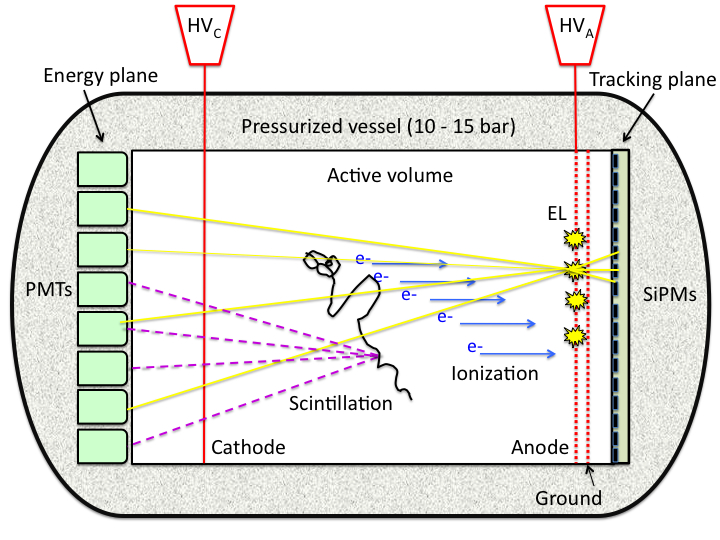
\includegraphics[width=0.49\textwidth]{img/SOFT.jpg}
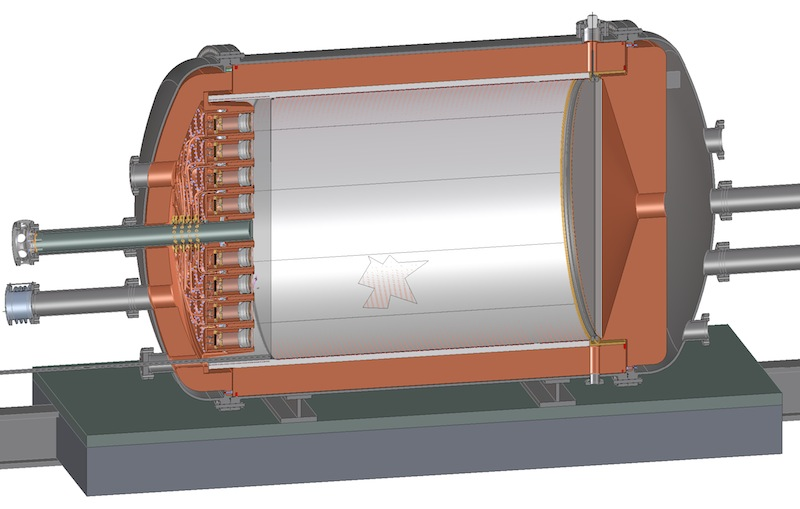
\includegraphics[width=0.49\textwidth]{img/NEXT100_full.jpg}
\caption{\small Left: The detection process in NEXT. Right: cross-section drawing of the NEXT-100 detector. The pressure vessel, 2.3 m long and 1.5 m diameter, can hold up to 150 kg of xenon at 15 bar.} \label{fig.SOFT}
\end{figure}
%%%%%%%%%%


The design of the NEXT-100 detector, shown in the right panel of Figure~\ref{fig.SOFT}, has been published in a \emph{Technical Design Report}.\footcite{Alvarez:2012haa} The construction of the detector ancillary systems (shielding, gas system, etcetera) is underway at the Laboratorio Subterr\'aneo de Canfranc (LSC), in Spain. 

NEXT-100 has the structure of a Matryoshka (a Russian nesting doll). The outermost layer is a shield made of lead, which attenuates the background from the LSC rock by 6 orders of magnitude (e.g, the \TL\ photons are attenuated from $\sim 10^{12}$~per year to $\sim 10^{6}$~per year). The pressure vessel, built out of steel, can hold 150 kg of xenon at 15 bar. Finally, an inner copper shield, 12 cm thick, constitutes the innermost and more radio-clean layer of the Matryoshka. All NEXT components have been selected and screened for low background. Of particular importance are the PMTs, whose activity is only 0.4 mBq of \BI\ and 0.3 mBq of \TL\ per unit. Our TDR shows a full quantification of the different contributions to the NEXT radioactive budget. A recent paper\footcite{Alvarez:2012as} quantifies the results of our screening campaign. Currently, most of the major components entering the NEXT detector have been measured, and those numbers are incorporated in our background model. 

%%%%%%%%%%%%%%%%%%%%%%%%%%%%%%%%%%%%%%%%%%%%%%%%%%%%%%%%%%%%
\subsubsection*{Prototypes}

%%%%%%%%%
\begin{figure}
\centering
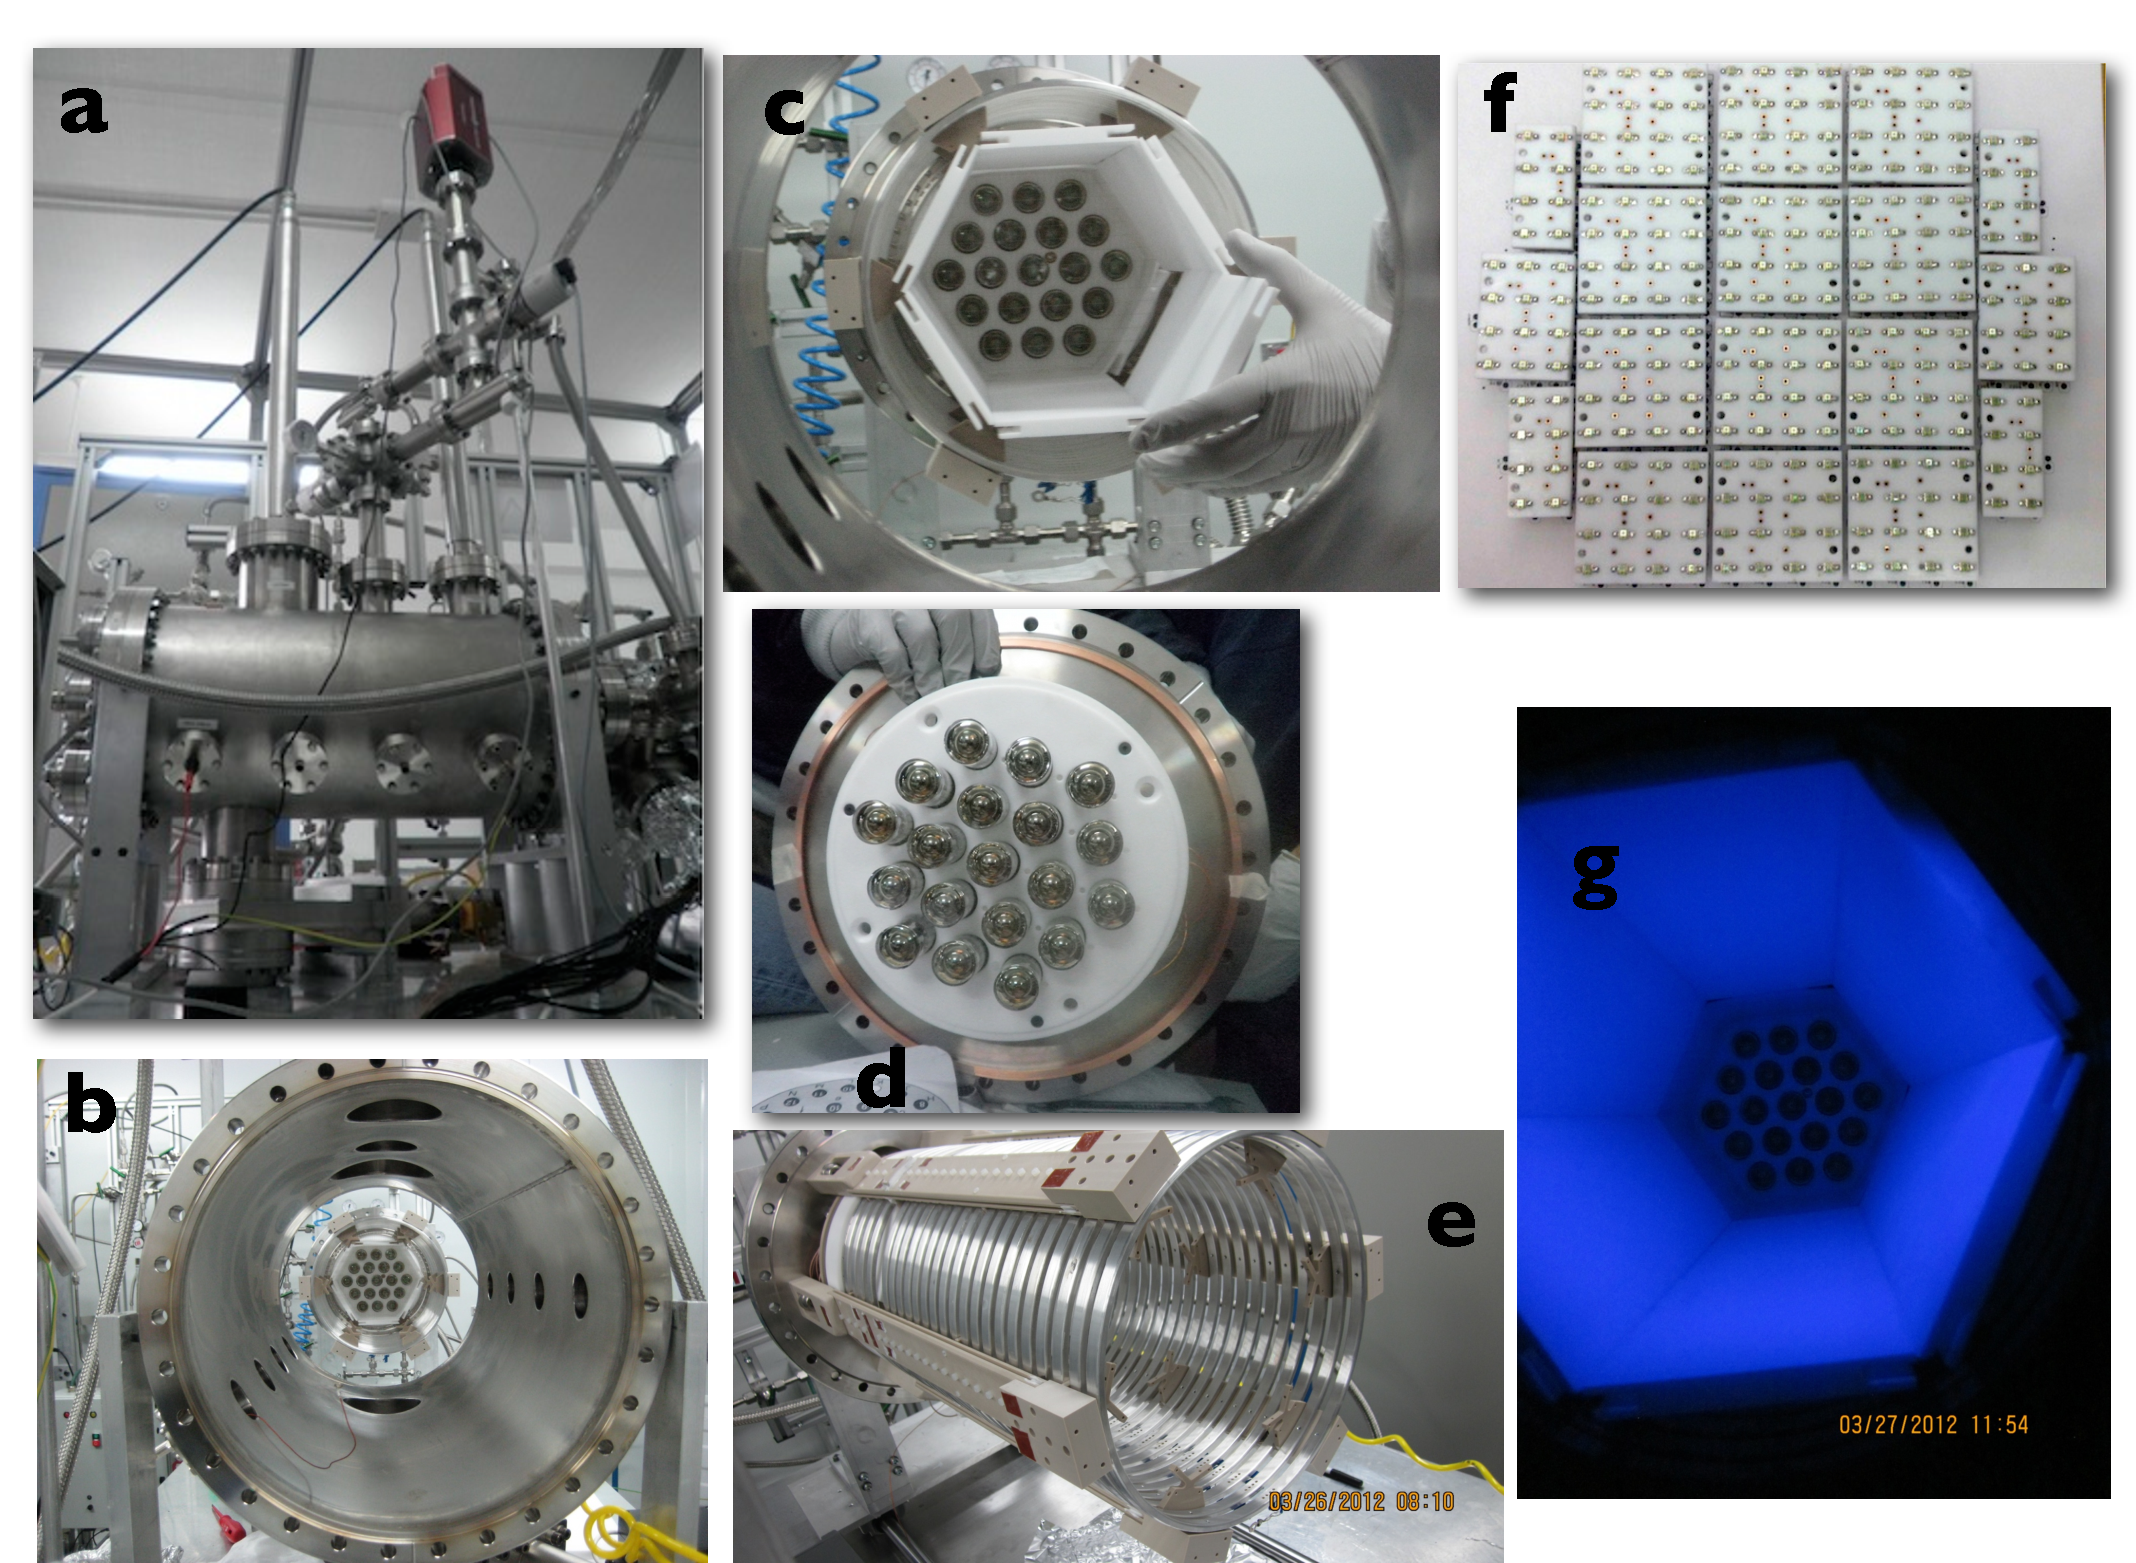
\includegraphics[width=0.7\textwidth]{img/DEMO.pdf}
\caption{\small The NEXT-DEMO prototype. (a) The pressure vessel, showing the HVFT and the mass spectrometer; (b) an expanded view of the detector; (c) Teflon light tube; (d) energy plane, made of pressure resistant Hamamatsu R7378A PMTs; (e) field cage; (f) tracking plane equipped with 300 Hamamatsu MPPCs; (g) Light tube coated with TPB, reflecting UV light in blue.} \label{fig.DEMO}
\end{figure}
%%%%%%%%%%

From 2009 to 2013 the NEXT Collaboration has carried out an intense R\&D program that has culminated in the construction, commissioning and operation of the NEXT-DEMO prototype located at IFIC, and the NEXT-DBDM prototype operating at LBNL. The description of these prototypes and the initial results obtained with them have recently been published\footcite{Alvarez:2012hh, Alvarez:2012nd, Alvarez:2012hu}.

NEXT-DEMO, shown in figure \ref{fig.DEMO}, is as a large-scale prototype and demonstrator of NEXT-100. The pressure vessel has a length of 60 cm and a diameter of 30 cm. The vessel can withstand a pressure of up to 15 bar. The maximum capacity of the detector is 10 kg but in its current configuration (the fiducial volume is an hexagon of 16 cm diameter and 30 cm length) it holds 4 kg at 15 bar. NEXT-DEMO is  equipped with an energy plane made of 19 Hamamatsu R7378A PMTs and a tracking plane made of 300 Hamamatsu MPPCs. 

The detector has been operating successfully for more than one year and has demonstrated: (a) very good operational stability, with no leaks and very few sparks; (b) good energy resolution ; (c) track reconstruction with PMTs and with SiPMs coated with TPB; (d) excellent electron drift lifetime, of the order of 20 ms. In summary, the operation of NEXT-DEMO has been instrumental in the development of the required knowledge to design and build the NEXT detector.

The NEXT-DBDM prototype is a smaller chamber, with only 8 cm drift, but an aspect ratio (ratio diameter to length) similar to the NEXT detector. The device has been used to perform detailed energy resolution studies. NEXT-DBDM achieves a resolution of 1\% FWHM at 660 keV and 15 bar, which extrapolates to 0.5\% at \Qbb.

\subsubsection*{Topological signature}

%%%%%
\begin{figure}
\centering
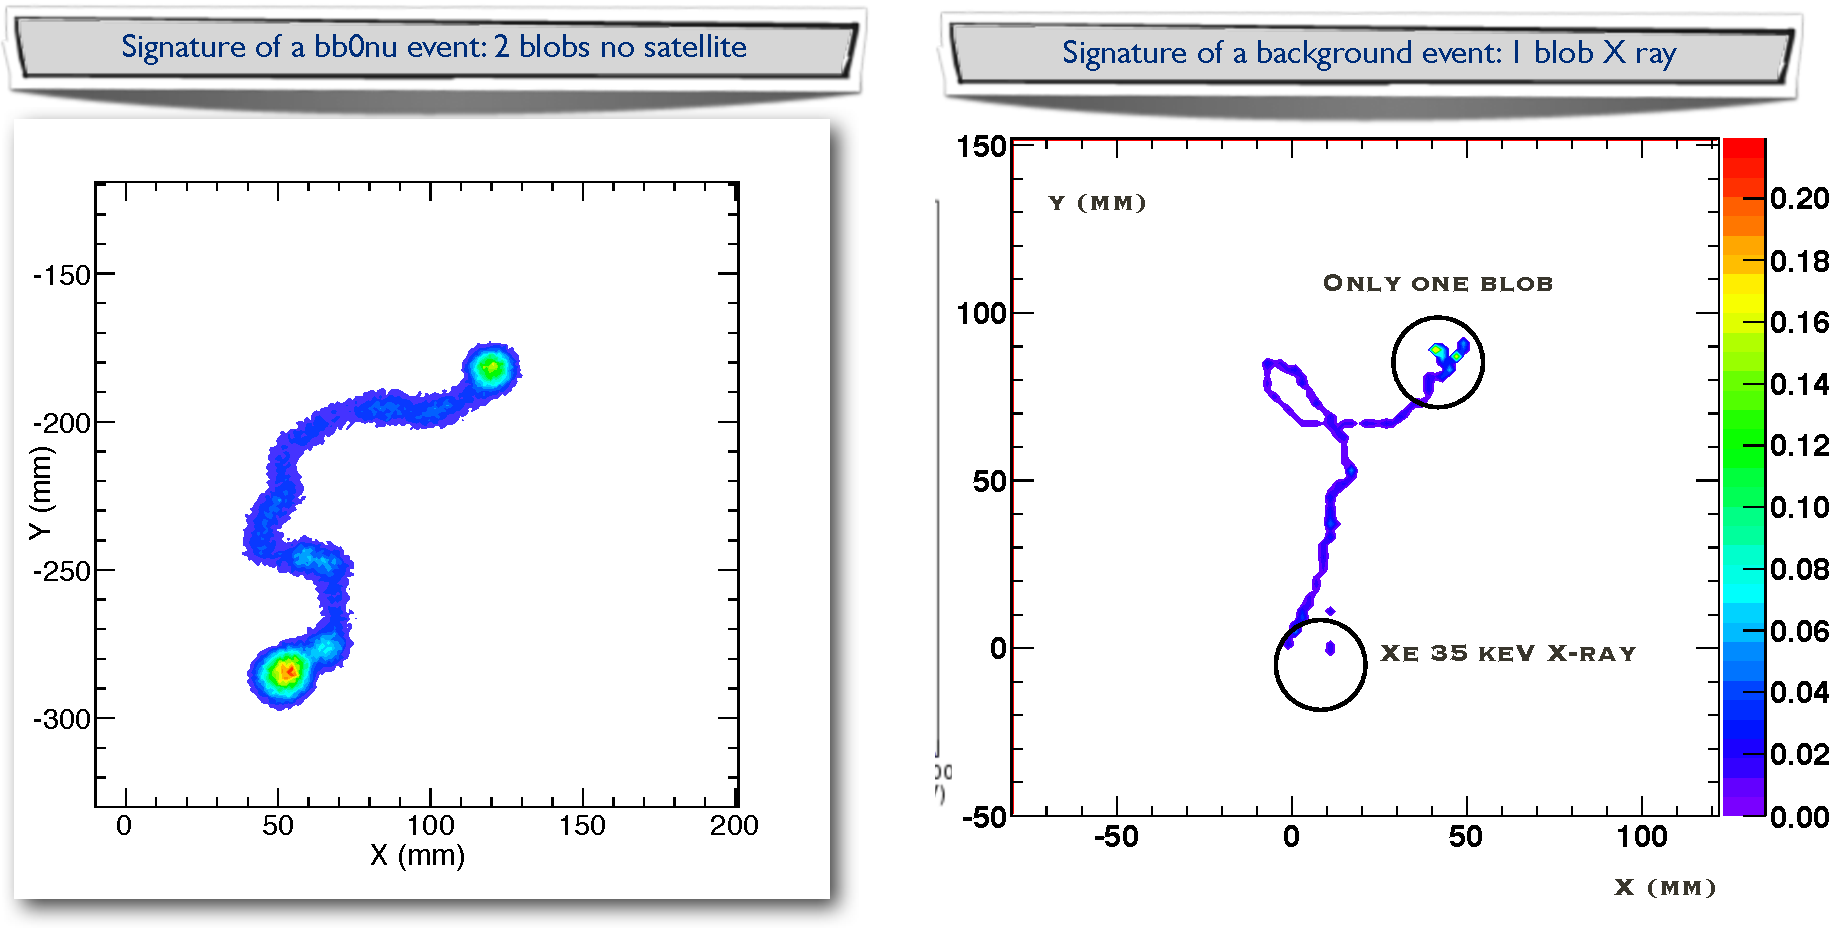
\includegraphics[width=0.9\textwidth]{img/ETRK2.pdf}
\caption{\small NEXT has a topological signature, not available in most \bbonu\ detectors. The panel shows the reconstruction of a Monte Carlo signal (left) and background (right) event. The signal has two electrons (two blobs). The background has only one electron (one blob) and the associated emission of a 35 keV X-ray. The color codes energy deposition in the TPC.}\label{fig.ETRK2}
\end{figure}
%%%%%
	
Double beta decay events leave a distinctive topological signature in HPXe: a continuous track with larger energy depositions (\emph{blobs}) at both ends due to the Bragg-like peaks in the d$E$/d$x$ of the stopping electrons (figure \ref{fig.ETRK2}, left). In contrast, background electrons are produced by Compton or photoelectric interactions, and are characterized by a single blob and, often, by a satellite cluster corresponding to the emission of $\sim30$-keV fluorescence x-rays by xenon (figure \ref{fig.ETRK2}, right).
Reconstruction of this topology using the tracking plane provides a powerful means of background rejection. In our TDR we chose a conservative cut to separate double--blob from single--blob events which provided a suppression factor of 20 for the background while keeping 80\% of the signal.  

The NEXT-DEMO prototype has demonstrated that electron tracks can be easily characterised in an HPXe TPC. Na-22 electrons, with an energy of 511 keV, have been used to demonstrate an efficiency of single-blob counting larger than 98\% and a frequency of erroneous double blob counting of less than 0.14\%. This is a robust confirmation of the excellent background rejection capability of the technology. 

\subsubsection*{Energy resolution}

%%%%%%
%\begin{figure}
%\centering
%\includegraphics[width=0.7\textwidth]{imgs2/RES.pdf}
%\caption{Energy resolution measured with NEXT-DBDM prototype at  15 bar. Data points show the measured energy resolution for 662 keV gammas (squares), 30 keV xenon X-rays (triangles) and LED light pulses (circles) as a function of the number of photons detected. The expected resolution including the intrinsic Fano factor, the statistical fluctuations in the number of detected photons and the PMT charge measurement variance. The measured resolution extrapolates to $\sim$0.5\% FWHM at \Qbb.}\label{fig.RES}
%\end{figure}
%%%%%

%%%%%
\begin{figure}
\centering
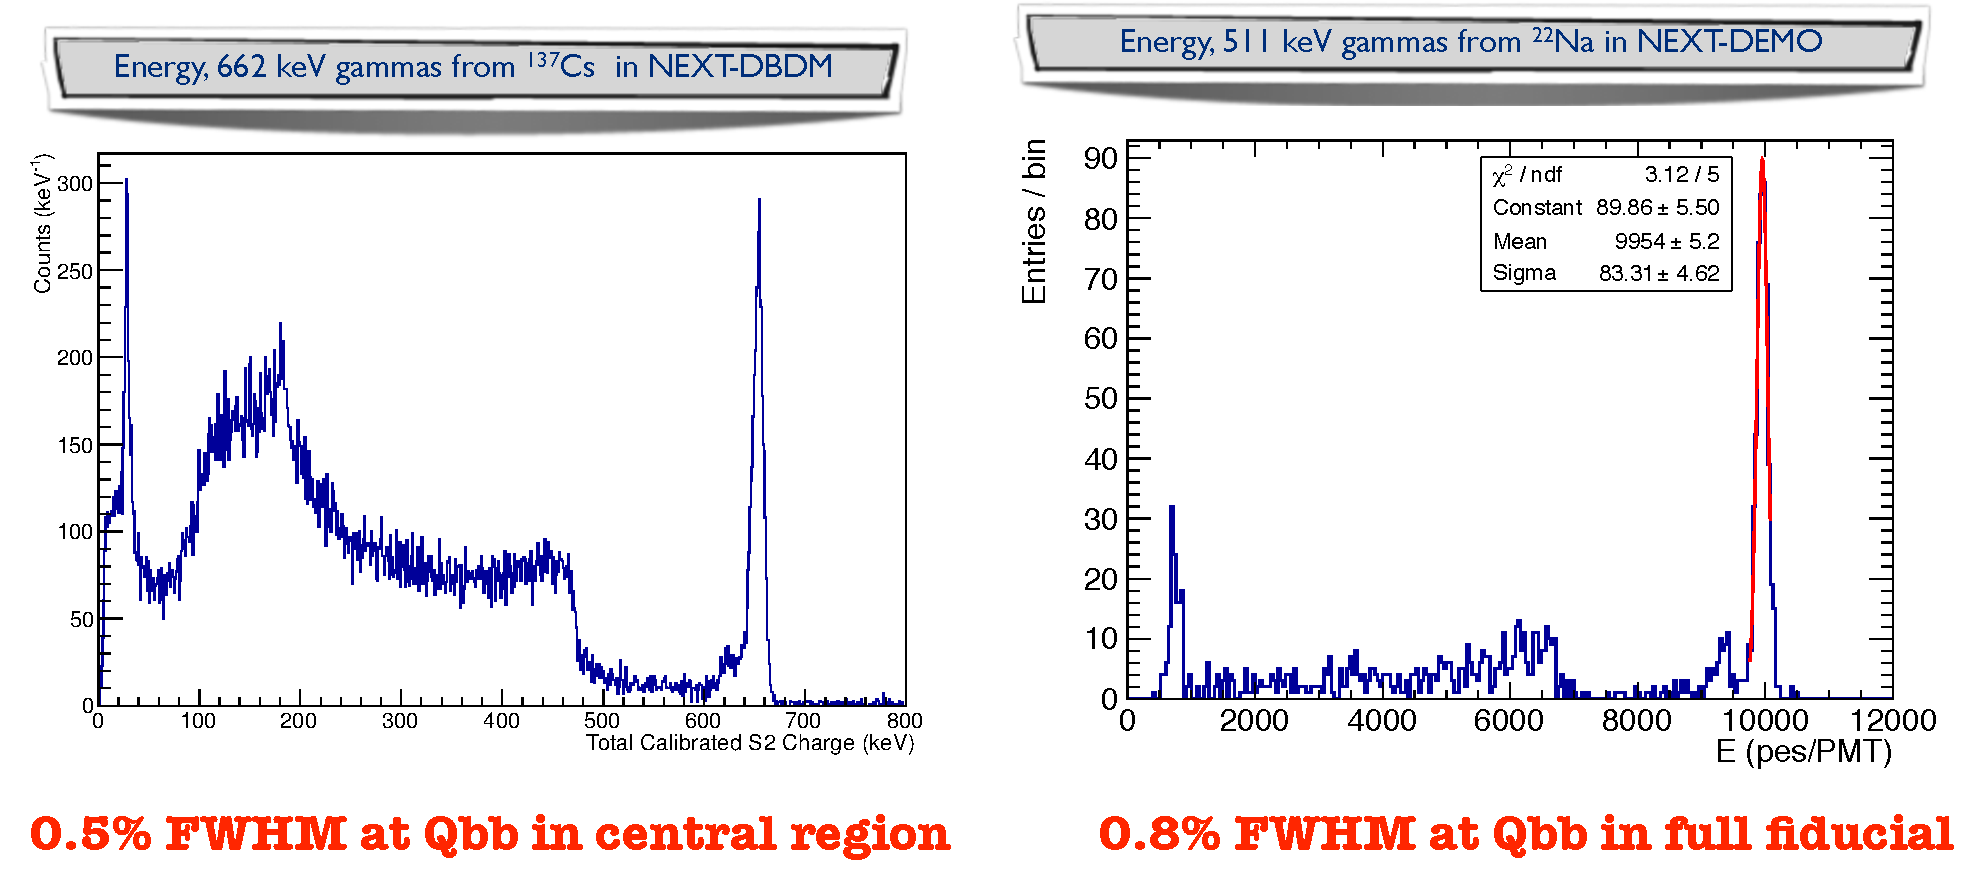
\includegraphics[width=0.9\textwidth]{img/ERS2.pdf}
\caption{\small Left: The resolution of the photo peak for 662 keV electrons in NEXT-DBDM, at 15 bar is 1\% FWHM (0.5\% FWHM at \Qbb); right panel: The resolution of the photo peak for 511 keV electrons in NEXT-DEMO, at 10 bar is 1.9\% FWHM (0.8\% FWHM at \Qbb).}\label{fig.ERES}
\end{figure}
%%%%

The resolution studies with the NEXT prototypes are summarized in Figure \ref{fig.ERES}. NEXT-DBDM apparatus has measured a resolution of 1\% FWHM with 
662 keV photons, which extrapolates to 0.5\% FWHM at \Qbb. This result is not far from the expected limit obtained adding in quadrature the different factors that contribute to the resolution (Fano factor, photoelectron statistics and electronic noise). It clearly shows that a resolution two times better than our initial target can be obtained. NEXT-DEMO measures a resolution of 1.8\% FWHM with 
511 keV photons, which extrapolates to 0.8\% FWHM at \Qbb. The fiducial volume of NEXT-DEMO is much larger than that of NEXT-DBDM and its aspect ratio (the ratio of diameter to length) is only 1/4 of the smaller prototype (whose aspect ratio is, however, close to that of NEXT-100). As a consequence, NEXT-DEMO collects about 3 times less light than NEXT-DBDM, a factor that enters photoelectron statistics and affects geometrical corrections. However, the resolution obtained by the larger prototype is already better than the target of 1\% FWHM described in the TDR.
\subsubsection*{Discovery potential}

%%%%%
\begin{figure}
\centering
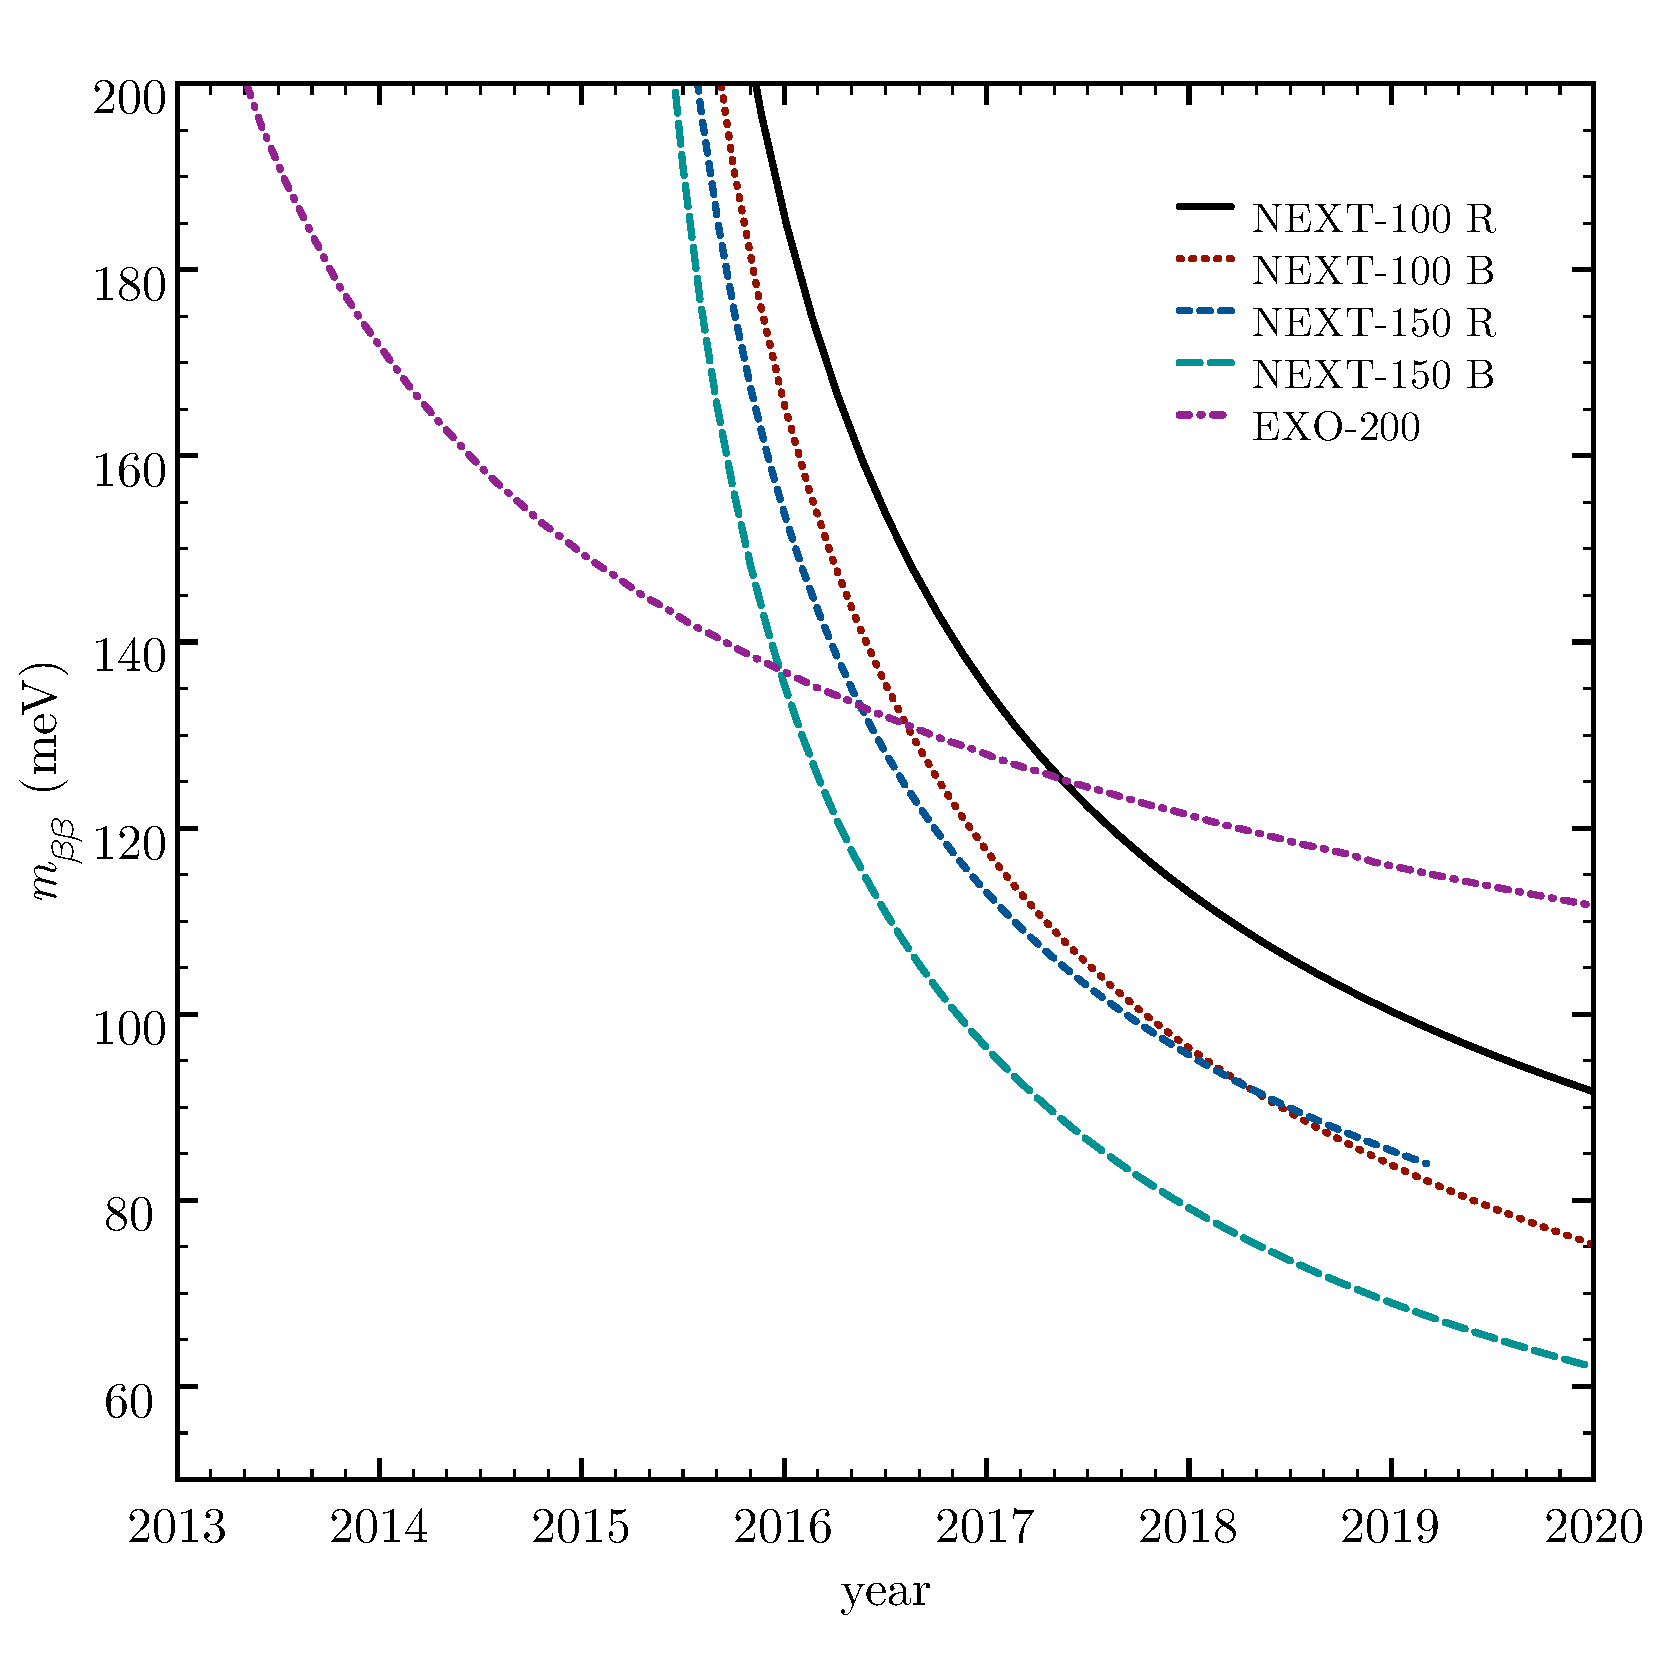
\includegraphics[width=0.5\textwidth]{img/EXOvsNEXT2.pdf}
\caption{Sensitivity of NEXT-100 assuming reference (R) and best (B) scenarios described in the text, as well as 100 and 150 kg of isotope mass.  The sensitivity of EXO-200 is drawn also for reference. It is assumed that the NEXT-100 \emph{physics run} starts in mid 2015.} \label{fig.exoNext}
\end{figure}
%%%%%

As shown in our TDR, the combination of excellent energy resolution and topological signature, results in a very good background rejection factor, estimated to be $\sim 2 \times 10^{-7}$~for the dominant background channels (the Bi-214 and Tl-208 
gammas of high energy entering the detector). NEXT-100 is a very radio-clean detector, protected by a thick shield of ultra radio pure copper, using ultra-radio pure PMTs and MPPCs. This, combined with the good background rejection factor, results in a very low background rate.

As a consequence, the discovery potential of NEXT is large. As explained below, we assume that the physics run starts in mid  2015, after detector commissioning in 2014. In our TDR we assumed a resolution of 1\% FWHM and quoted a background rate of $8 \times 10^{-4}$~\ckky, obtained from a detailed Monte Carlo calculation using our full background model. Since publication of the TDR our prototypes have measured better resolution than that assumed. DEMO reaches 0.8\% FWHM in a large fiducial volume, while DBDM reaches 0.5\% in a more restricted fiducial region. Moreover, the background model is fully backed by an extensive screening campaign that has fully quantified the radioactivity of all the components entering the detector\footcite{Alvarez:2012as}.

Indeed, as explained in the next sections, we believe that both figures can be improved. We aim, as a part of the research program described in this proposal, to achieve a resolution of 0.5\% FWHM at \Qbb, in the full fiducial region and a background rate of 
$2 \times 10^{-4}$~\ckky. The possibility exists to operate the detector with 100 kg of Xe-136 (already available) at 10 bar, or with 150 kg of Xe-136 at 15 bar.

Figure \ref{fig.exoNext} shows the sensitivity of NEXT-100 from the start of physics data taking under four scenarios: (a) reference,  with the conservative parameters assumed in the TDR and 100 kg of isotope in the chamber; (b) reference, with 150 kg of xenon; (c)  best, with the improved parameters described above and 100 kg of xenon; (d) best with  150 kg of isotope. For reference, we also consider the sensitivity of EXO-200, assuming the parameters described in the recent publication \footcite{Auger:2012ar}. 

Notice that the discovery potential of NEXT-100, in particular with 150 kg and/or the improved parameters is very high. Currently, EXO-200 and KamLAND-Zen are dominated by backgrounds and therefore, further data taking without detector improvement will yield a slow improvement in their results. Thus, in spite of a relatively late start, NEXT could quickly become competitive.  On the other hand, if GERDA, EXO-200, KamLAND-Zen
or another experiment (such as CUORE) were to claim a discovery in the next few years, NEXT would be in the perfect position to provide an independent confirmation.  

\subsubsection*{Towards a ton-scale HPGXe TPC}

%%%%%%
%\begin{figure}
%\centering
%\includegraphics[width=0.65\textwidth]{imgs2/SensitivityFuture.pdf}
%\caption{The sensitivity of NEXT versus that of EXO in the 1-ton regime.} \label{fig.NextFuture}
%\end{figure}
%%%%%%

If no discovery is made by the current generation of experiments, the full exploration of the inverse hierarchy of neutrino masses requires detectors of larger mass (at least 1 ton), with good energy resolution and extremely low specific background. With a resolution of 0.5\% FWHM and a background rate of $2 \times 10^{-4}$\ckky, as we intend to demonstrate in this research, an HPXe detector with a mass in the ton scale could fully explore the inverse hierarchy. %The discovery potential is, therefore, enormous. 

In that sense, NEXT is the perfect springboard for a detector in the ton scale. The resolution and background rate described in our TDR would allow a detector of 100-150 kg to reach sensitivities in the range of 50-100 meV, but the improved parameters that we expect to reach after our R\&D, would demonstrate that the HPXe gas technology can fully explore the inverse hierarchy. 

Taking into account that EXO-200 operates in USA and Kamland-Zen operates in Japan, the NEXT program offers a unique opportunity for Europe to lead with the HPXe technology. This would make Europe a major player in the area of xenon detectors applied to \bbonu. This is particularly relevant, since xenon will very likely be the easiest isotope to reach the ton scale.
 
